
\documentclass[article]{llncs}
%
\usepackage[utf8]{inputenc}
\usepackage[spanish]{babel}
\usepackage{graphicx}
% Used for displaying a sample figure. If possible, figure files should
% be included in EPS format.
%
% If you use the hyperref package, please uncomment the following line
% to display URLs in blue roman font according to Springer's eBook style:
% \renewcommand\UrlFont{\color{blue}\rmfamily}


\begin{document}
%
\title{Detecci\'on de Instalaciones con Machine Learning}
%
%\titlerunning{Abbreviated paper title}
% If the paper title is too long for the running head, you can set
% an abbreviated paper title here
%
\author{Jes\'us Santos Capote, Kenny Villalobos Morales, Jorge Soler Gonz\'alez, Abraham Gonz\'alez Rivero, 
Rainel Fern\'andez Abreu, Eduardo Garc\'ia Maleta}
%
\institute{Facultad de Matemática y Computación, Universidad de La Habana, La Habana, Cuba }
%
\maketitle              % typeset the header of the contribution
%

\keywords{Detección de Objetos \and Clasificación de Im\'agenes \and Machine Learning \and Pytorch \and Keras \and Tensorflow \and Faster-RCNN}


\section{Intoducci\'on}
El uso de imágenes satelitales ha permitido avances significativos en la identificación y caracterización de diferentes 
tipos de construcciones, lo cual puede ser de gran utilidad en diversas áreas como la planificación urbana, la gestión de 
recursos naturales y la seguridad nacional, entre otras. Los autores proponen cuatro modelos, dos de clasificación de im\'agenes, 
uno de detección de objetos y uno segmentaci\'on con el fin de identificar en im\'agenes satelitales edificaciones con una topolog\'ia espec\'ifica.

\section{Estado del Arte}
Actualmente para resolver la problemática se utilizan técnicas de aprendizaje profundo, específicamente 
redes neuronales convolucionales, para la detección y clasificación de edificios e instalaciones en imágenes de 
teledetección y satélite. Estas redes neuronales convolucionales permiten extraer características relevantes de las imágenes 
y clasificarlas en diferentes categorías.

Algunos artículos utilizan técnicas de reducción de dimensionalidad, como Análisis de Componentes Principales 
(PCA), para extraer características de las imágenes y reducir la complejidad de las mismas. PCA selecciona las 
características más importantes de la imagen y las utiliza para entrenar el modelo de aprendizaje profundo, lo que 
acelera el proceso de entrenamiento y mejora la precisión.

Otra técnica utilizada es la transferencia de aprendizaje para mejorar el rendimiento de las redes neuronales. Esta 
técnica implica reutilizar una red previamente entrenada en una tarea relacionada para una nueva tarea. 
Al utilizar el conocimiento previo adquirido en la tarea anterior, el modelo puede aprender más rápido y mejorar 
su precisión.

Otros utilizan técnicas de filtrado guiado para mejorar la calidad de la solución. Esta técnica utiliza una 
imagen guía de alta calidad para filtrar una imagen de baja calidad y mejorar la resolución y la claridad de la imagen.

La optimización estructurada también se emplea en algunos artículos para mejorar la precisión de la segmentación de 
edificios. Esta técnica utiliza restricciones estructurales para mejorar la coherencia y la continuidad de los 
objetos segmentados, lo que puede mejorar la precisión y la calidad de la solución.

Otro enfoque utilizado es la combinación de varias de estas técnicas. Algunos autores utilizan algoritmos de clustering 
para el procesamiento de las imágenes y encontrar patrones en estas, los algoritmos más usados son el K-Means y Mean Shift. Otras de las más combinadas 
son la reducción de dimensiones con PCA y redes neuronales convolucionales.

Ross Girshick en su artículo "Fast R-CNN" hace una propuesta de una nueva técnica \cite{FRCNN}. Fast R-CNN utiliza una red neuronal 
convolucional para extraer características de la imagen y una capa de regresión para localizar objetos en la imagen. 
A diferencia de "R-CNN", "Fast R-CNN" utiliza una sola red convolucional para extraer características de la imagen y 
detectar objetos, lo que mejora la eficiencia computacional y la velocidad de procesamiento. Su eficiencia computacional y su alta precisión en la detección de objetos 
lo hacen una técnica atractiva, por lo que nuestro modelo principal se basa en esta. 

En el artículo "Satellite Image Classification with Deep Learning" \cite{satelite}, se ve un enfoque donde primeramente se 
preprocesan las imágenes para posteriormente brindarselas a una CNN, alargando los bordes de las cajas donde se encuentran los objetos en proporción con el tamaño de 
la imagen, este paso es necesario porque provee de un contexto de píxeles alrededor del objeto que son de interés para la red 
neuronal. Además el modelo CNN que utilizan trae consigo 4 arquitecturas (DenseNet, ResNet, Inception, Xception). 
Dado que el enfoque de este artículo tiene una alta precisión en la problemática que se trata y está explicado con bastante claridad 
se decidió usarlo en uno de los modelos implementados.

Recientemente se está trabajando en un modelo llamado Segment Anything Model (SAM) \cite{SAM}, que es particularmente útil 
en el campo de la detección y la clasificación de instalaciones en imágenes satelitales. Dada su fiabilidad usamos 
este modelo para comparar sus resultados con los implementados por nosotros.




\section{Dataset}

\subsection{Functional Map of the World Dataset}

El dataset usado para el entrenamiento de los modelos fue el llamado Functional Map of the World Dataset. 
El conjunto de datos "Functional Map of the World" (FMOW) es un conjunto de datos público de imágenes satelitales 
que se utiliza para tareas de clasificación de objetos y detección de objetos. El conjunto de datos contiene alrededor 
de 1 millón de imágenes de alta resolución de todo el mundo, que se han etiquetado manualmente con información sobre 
las clases de objetos presentes en la imagen.

El FMOW se divide en dos partes principales: una parte de entrenamiento y una parte de prueba. La parte de entrenamiento 
consta de alrededor de 900,000 imágenes etiquetadas, mientras que la parte de prueba contiene alrededor de 100,000 
imágenes no etiquetadas. Las imágenes en el conjunto de datos muestran una variedad de paisajes y entornos, incluidas 
áreas urbanas y rurales, y se capturaron en diferentes momentos del día y en diferentes condiciones climáticas.

Las etiquetas de clase en el FMOW se basan en una taxonomía de objetos llamada "Functional Map of the World" (FMoW). La 
taxonomía FMoW se centra en las funciones que cumplen los objetos en lugar de en su apariencia física, lo que permite 
una clasificación más precisa y consistente de los objetos en diferentes contextos y entornos. Las clases de objetos 
incluyen cosas como edificios, vehículos, cuerpos de agua, cultivos y áreas verdes.

Actualmente se encuentra libre para su descarga en Amazon S3.

\subsection{Cuba Stadia}

Este es un dataset creado por el equipo para el entrenamiento y pruebas de los modelos implementdos. Consta de 38 
im\'agenes de estadios de beisbol de nuestro territorio nacional con sus correspondientes etiquetas. Cada etiqueta 
contiene el Bounding Box del estadio as\'i como las dimensiones de la im\'agen. Se construy\'o tomando screenshots 
de Google Maps Satelital, sin etiquetas, luego he recortado las imagenes en forma cuadrada con 720 pixeles de ancho. 
Las anotaciones fueron realizadas con una aplicaci\'on de nuestra autor\'ia.

\section{Modelos Utilizados}

\subsection{Faster R-CNN}
Faster R-CNN es un algoritmo popular de detección de objetos que fue introducido por Shaoqing Ren, 
Kaiming He, Ross Girshick y Jian Sun en 2015. Es una extensión del modelo R-CNN original (Convolutional Neural 
Network basado en regiones), que fue introducido por Ross Girshick et al. en 2014.

La detección de objetos con Faster-RCNN se logra primero generando un conjunto de propuestas de región 
(es decir, ubicaciones de objetos candidatos) utilizando una Red de Proposición de Regiones (RPN), y luego 
clasificando estas propuestas utilizando una red de clasificación.

La RPN es una red neuronal completamente convolucional que toma una imagen como entrada y produce un conjunto de 
propuestas de objetos rectangulares, cada una con una puntuación de objetividad asociada. Estas propuestas se generan 
deslizando una pequeña red sobre el mapa de características convolucionales producido por una red de base pre-entrenada 
(típicamente una red VGG o ResNet). La RPN se entrena de extremo a extremo con la red de clasificación, utilizando una 
función de pérdida de múltiples tareas que combina una pérdida de clasificación binaria para la objetividad y una 
pérdida de regresión para las coordenadas del cuadro delimitador.

La red de clasificación toma cada propuesta generada por la RPN y realiza la clasificación de objetos y la regresión 
del cuadro delimitador. La red consta de una serie de capas completamente conectadas que toman las características de 
cada propuesta como entrada y producen una etiqueta de clase y coordenadas del cuadro delimitador.

La implementaci\'on de este modelo se realiz\'o con la utilizaci\'on de la biblioteca Pytorch de python y se realiz\'o el
entranmiento en Google Colab con la clase Stadium del dataset. Es decir el modelo se entren\'o para detectar estadios en 
im\'agenes satelitales. De igual forma se puede entrenar para detectar otro tipo de edificaci\'on.

\subsection{InceptionV3 + DNN}

El modelo de machine learning que se presenta utiliza la arquitectura InceptionV3 de redes neuronales convolucionales 
(CNN) para la extracción de características, seguida de una red neuronal densa (DNN) para la clasificación.

El modelo InceptionV3 es una red neuronal convolucional profunda que ha demostrado ser altamente eficaz en la 
clasificación de imágenes. Fue desarrollado por Google y se encuentra disponible en la librería de aprendizaje profundo 
Keras, lo que lo hace accesible para su uso en proyectos de Machine Learning.

El modelo InceptionV3 se caracteriza por su arquitectura en forma de "inception module", que se basa en la idea de 
combinar diferentes tamaños de filtros dentro de la misma capa convolucional. Esta técnica permite reducir la cantidad 
de parámetros que debe aprender el modelo, lo que a su vez reduce el riesgo de sobreajuste y mejora su capacidad de 
generalización.

Además, InceptionV3 utiliza técnicas como la regularización L2 y el dropout para prevenir el sobreajuste, y utiliza la 
función de activación ReLU para acelerar el entrenamiento de la red. El modelo también utiliza capas de agrupamiento 
máximo (max pooling) para reducir el tamaño de las características de la imagen y facilitar su procesamiento.

La red neuronal densa que se agrega a la arquitectura InceptionV3 se utiliza para la clasificación de las características 
extraídas por la red convolucional. La red consta de dos capas densas completamente conectadas con 128 y 2 neuronas respectivamente. 
La capa final de la red densa utiliza la función de activación softmax, que normaliza 
las salidas de la capa anterior para que representen probabilidades de clase para la clasificación multiclase. La función 
de activación ReLU se utiliza en la capa anterior para introducir no linealidad en la red y mejorar su capacidad de 
aprendizaje.

El modelo se entren\'o para la clasificación de im\'agenes con aeropuertos y zool\'ogicos.


\subsection{DenseNet + ResNet + InceptionV3 + Xception}

Este es un modelo de aprendizaje profundo que utiliza cuatro arquitecturas de redes neuronales pre-entrenadas 
(DenseNet121, ResNet152, InceptionV3 y Xception) para extraer características de una imagen de entrada de tamaño 
224x224x3 y luego combinar estas características en una capa de fusión. La salida de la capa de fusión se alimenta a 
través de una capa densa completamente conectada con 1024 unidades y una función de activación ReLU, seguida de una capa 
de dropout para reducir el sobreajuste. Finalmente, hay una capa densa con una función de activación softmax que predice 
la probabilidad de pertenecer a cada una de las clases de destino.

DenseNet121: DenseNet es una arquitectura de red neuronal convolucional profunda que se caracteriza por tener conexiones 
densas entre las capas. DenseNet121 es una versión específica de esta arquitectura que tiene 121 capas y se ha entrenado 
en un conjunto de datos masivo llamado ImageNet. Esta arquitectura es conocida por su eficiencia y precisión en la 
clasificación de imágenes.

ResNet152: ResNet es otra arquitectura de red neuronal convolucional profunda que se caracteriza por tener conexiones 
residuales entre las capas. Estas conexiones permiten que la información fluya directamente a través de la red, lo que 
facilita el entrenamiento de redes más profundas. ResNet152 es una versión específica de esta arquitectura que tiene 152 
capas y también se ha entrenado en el conjunto de datos ImageNet. Esta arquitectura ha demostrado ser muy eficaz para 
tareas de clasificación de imágenes.

InceptionV3: Inception es una arquitectura de red neuronal convolucional que se caracteriza por tener múltiples caminos 
de procesamiento de información dentro de la red. InceptionV3 es una versión específica de esta arquitectura que se ha 
entrenado en el conjunto de datos ImageNet. Esta arquitectura es conocida por su eficiencia y precisión en la 
clasificación de imágenes.

Xception: Xception es una arquitectura de red neuronal convolucional profunda que se caracteriza por tener convoluciones 
separables en profundidad. Las convoluciones separables en profundidad son una variante de las convoluciones regulares 
que separan el procesamiento espacial y de características en dos etapas diferentes. Xception se ha entrenado en el 
conjunto de datos ImageNet y ha demostrado ser muy eficaz para tareas de clasificación de imágenes.

EL modelo fue entrenado para identificar las clases: airport terminal, burial site, park, stadium, zoo.

\subsection{Segmentaci\'on con K-Means}

Se experiment\'o con cuatro propuestas de algoritmos que utilizan K-Means para segmentar las im\'agenes satelitales:

\subsubsection{K-Means sobre p\'ixeles:}
Se aplica el algoritmo de K-Means sobre los valores RGB de los p\'ixeles de la im\'agen satelital. Las edificaciones, 
en su mayor\'ia tienen un mismo color, por tanto un agrupamiento de los p\'ixeles por colores similares puede segmentar 
las edificaciones presentes en la im\'agen.

\subsubsection{K-Means sobre RGB y coordenads XY:}
Mejorando la propuesta anterior, por cada p\'ixel hay un vector de 5 componentes 
que contiene los valores RGB y las coordenadas XY de cada p\'ixel. A estos vectores se les aplica el algoritmo de clustering. Incluir 
las coordenadas XY del p\'ixel permite que la agrupaci\'on tenga en cuenta no solo el color sino también la cercan\'ia 
entre los p\'ixeles. 

\subsubsection{K-Means y Algoritmo de Canny:}
El algoritmo de Canny es un algoritmo de detección de bordes ampliamente utilizado en el procesamiento de imágenes. 
El resultado de aplicarlo es una imagen binaria que contiene los bordes detectados en la imagen original. Se aplica 
K-Means a la im\'agen satelital y se superponen las imagenes resultantes de aplicar Canny y K-Means para obtener la segmentacion.

La selecci\'on del par\'ametro K del algortimo K-Means se efect\'ua mediante el m\'etodo del codo. 

\section{Conclusiones}
Los resultados obtenidos son prometedores dado que solo se usan im\'agenes en RGB y todos los resultados importantes 
sobre el tema abordado utilizan im\'agenes multiespectrales. El modelo principal del trabajo, Faster R-CNN  
obtiene como valor promedio, 0.4 en la m\'etrica Mean Average Presition(mAP), detectando instancias de estadios. Valor 
algo discreto en comparación a los resultados del Estado de Arte. 

Los autores concluyen que las t\'ecnicas de aprendizaje no supervisado, por si solas, no son las m\'as apropiadas 
para enfrentar los problemas de detección de objetos en im\'agenes satelitales. Los algoritmos de clustering implementados 
proveen resultados prometedores, aunque no tan descriptivos y pr\'acticos como los algoritmos supervisados implementados.

\section{Resultados}

Ver figuras 1, 2, 3, 4

% \begin{figure}[h]
%   \centering
%   \includegraphics[width=0.5\textwidth]{estadio_guillermon_moncada.jpg}
%   \caption{Imagen Original: Estadio Guillerm\'on Moncada}
%   \label{fig:estadio_guillermon_moncada}
% \end{figure}

\begin{figure}[h]
  \centering
  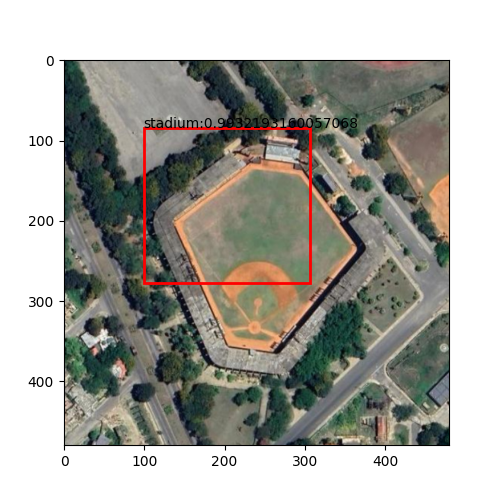
\includegraphics[width=0.5\textwidth]{Figure_1.png}
  \caption{Predicci\'on de Faster-RCNN}
  \label{fig:Figure_1}
\end{figure}

\begin{figure}[h]
  \centering
  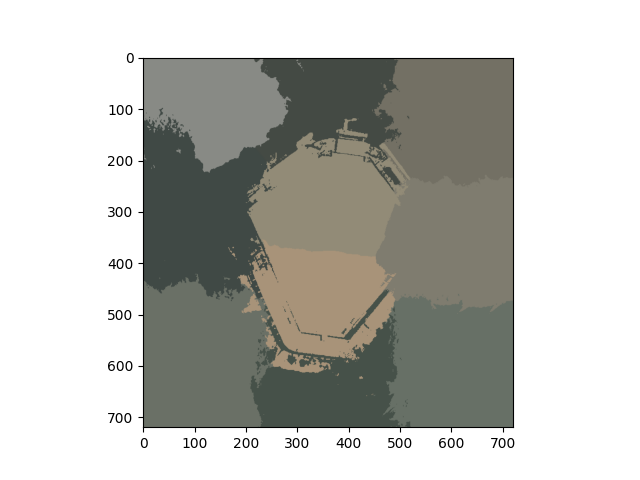
\includegraphics[width=0.5\textwidth]{Figure_2.png}
  \caption{K-Means RGB + XY}
  \label{fig:Figure_2}
\end{figure}

\begin{figure}[h]
  \centering
  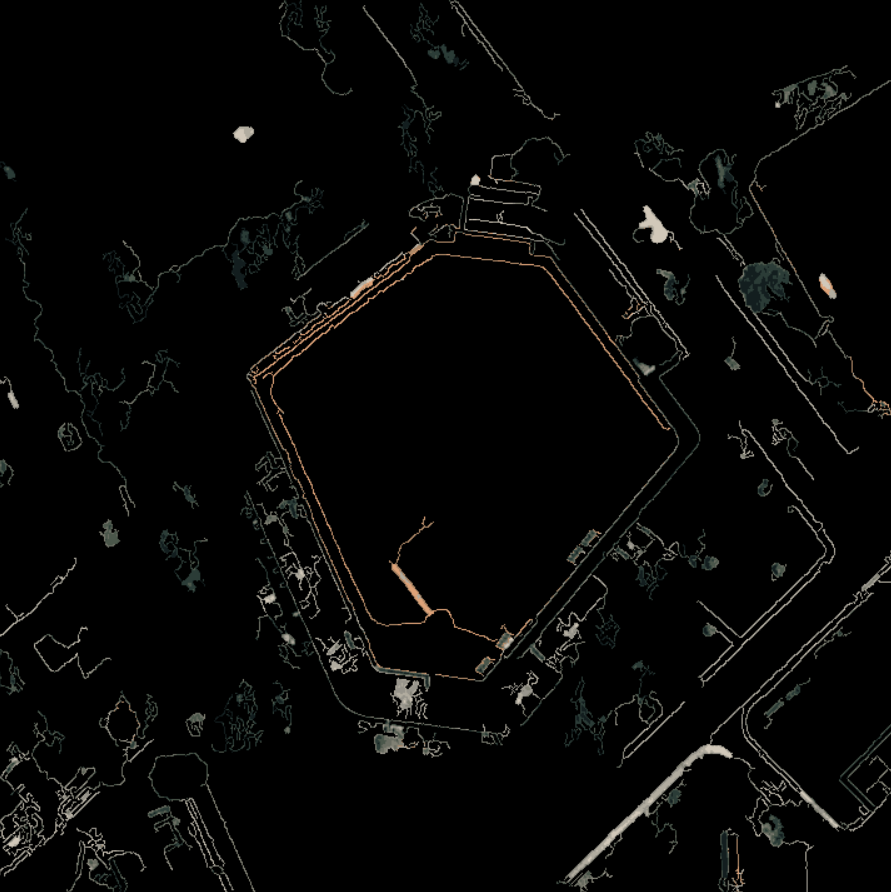
\includegraphics[width=0.5\textwidth]{canny.png}
  \caption{K-Means + Canny}
  \label{fig:canny}
\end{figure}

\begin{thebibliography}{8}
    \bibitem{citekey}
        K. He et al., “Deep residual learning for image recognition,” arXiv 1512.03385, Dec 2015.
  
    \bibitem{citekey}
        G. Huang, “Dense connected convolutional neural networks,” IEEE Computer Society Conference on Computer Vision and Pattern Recognition (CVPR), 2017.
    
    \bibitem{citekey}
        Ishii, Tomohiro, Edgar Simo-Serra, Satoshi Iizuka, Yoshihiko Mochizuki, Akihiro Sugimoto, Hiroshi Ishikawa, y Ryosuke Nakamura. «Detection by classification of buildings in multispectral satellite imagery». En 2016 23rd International Conference on Pattern Recognition (ICPR), 3344-49, 2016. https://doi.org/10.1109/ICPR.2016.7900150.
    
    \bibitem{satelite}
        Pritt, Mark, y Gary Chern. «Satellite Image Classification with Deep Learning». En 2017 IEEE Applied Imagery Pattern Recognition Workshop (AIPR), 1-7, 2017. https://doi.org/10.1109/AIPR.2017.8457969.

    \bibitem{citekey}
        Reda, Kinga, y Michal Kedzierski. «Detection, Classification and Boundary Regularization of Buildings in Satellite Imagery Using Faster Edge Region Convolutional Neural Networks». Remote Sensing 12, n.º 14 (enero de 2020): 2240. https://doi.org/10.3390/rs12142240.

    \bibitem{citekey}
        Christian Szegedy, Wei Liu, Yangqing Jia, Pierre Sermanet, Scott Reed, Dragomir Anguelov, Dumitru Erhan, Vincent Vanhoucke, and Andrew Rabinovich. "Going Deeper with Convolutions." Proceedings of the IEEE Conference on Computer Vision and Pattern Recognition (CVPR), 2015. doi: 10.1109/CVPR.2015.7298594

    \bibitem{citekey}
        François Chollet. "Xception: Deep Learning with Depthwise Separable Convolutions." Proceedings of the IEEE Conference on Computer Vision and Pattern Recognition (CVPR), 2017. doi: 10.1109/CVPR.2017.195

    \bibitem{citekey}
        W. Shao, "Unsupervised feature learning for urban land use classification using deep convolutional neural networks", ISPRS Journal of Photogrammetry and Remote Sensing, 2016
        
    \bibitem{FRCNN}
        Girshick Ross, "Fast R-CNN", En 2015 ICCV. https://arxiv.org/abs/1504.08083
      
    \bibitem{SAM}
        https://encord.com/blog/segment-anything-model-explained/\#h3

    \bibitem{citekey}
        Wenzhi Zhao; Shihong Du, "Spectral-Spatial Feature Extraction for Hyperspectral Image Classification: A Dimension Reduction and Deep Learning Approach", En 2016 IEEE Transactions on Geoscience and Remote Sensing, https://ieeexplore.ieee.org/abstract/document/7450160

    \bibitem{citekey}
        Adriana Romero; Carlo Gatta; Gustau Camps-Valls, "Unsupervised Deep Feature Extraction for Remote Sensing Image Classification", en 2016 IEEE Transactions on Geoscience and Remote Sensing, https://ieeexplore.ieee.org/document/7293195
    
    \bibitem{citekey}
        Aaron Reite, Scott Kangas, Zackery Steck, Steven Goley, Jonathan Von Stroh, Steven Forsyth, "Unsupervised Feature Learning in Remote Sensing", en 2019 https://arxiv.org/abs/1908.02877

    \bibitem{citekey}
        Tomohiro Ishii; Edgar Simo-Serra; Satoshi Iizuka; Yoshihiko Mochizuki; Akihiro Sugimoto; Hiroshi Ishikawa; Ryosuke Nakamura, "Detection by classification of buildings in multispectral satellite imagery", en 2016 23rd International Conference on Pattern Recognition (ICPR), https://ieeexplore.ieee.org/document/7900150
    
    \bibitem{citekey}     
        Dixit, M., Chaurasia, K., Mishra, V.K. (2021). Automatic Building Extraction from High-Resolution Satellite Images Using Deep Learning Techniques. In: Dave, M., Garg, R., Dua, M., Hussien, J. (eds) Proceedings of the International Conference on Paradigms of Computing, Communication and Data Sciences. Algorithms for Intelligent Systems. Springer, Singapore. $https://doi.org/10.1007/978-981-15-7533-4_61$
        
    \bibitem{citekey}
        M M Zhu, Y L Xu, S P Ma, H Q Ma, "Airport Detection on Remote Sensing Images Using Fater Region-based Convolutional Neural Network", Journal of Physics: Conference Series, vol.1060, pp.012037, 2018. https://iopscience.iop.org/article/10.1088/1742-6596/1060/1/012037/meta

    



  \end{thebibliography}

\end{document}